%%%%%%%%%%%%  Generated using docx2latex.com  %%%%%%%%%%%%%%

%%%%%%%%%%%%  v2.0.0-beta  %%%%%%%%%%%%%%

%\documentclass[12pt]{report}
%\usepackage{amsmath}
%\usepackage{latexsym}
%\usepackage{amsfonts}
%\usepackage[normalem]{ulem}
%\usepackage{array}
%\usepackage{amssymb}
%\usepackage{graphicx}
%\usepackage[backend=biber,
%style=numeric,
%sorting=none,
%isbn=false,
%doi=false,
%url=false,
%]{biblatex}\addbibresource{bibliography.bib}

%\usepackage{subfig}
%\usepackage{wrapfig}
%\usepackage{wasysym}
%\usepackage{enumitem}
%\usepackage{adjustbox}
%\usepackage{ragged2e}
%\usepackage[svgnames,table]{xcolor}
%\usepackage{tikz}
%\usepackage{longtable}
%\usepackage{changepage}
%\usepackage{setspace}
%\usepackage{hhline}
%\usepackage{multicol}
%\usepackage{tabto}
%\usepackage{float}
%\usepackage{multirow}
%\usepackage{makecell}
%\usepackage{fancyhdr}
%\usepackage[toc,page]{appendix}
%\usepackage[hidelinks]{hyperref}
%\usetikzlibrary{shapes.symbols,shapes.geometric,shadows,arrows.meta}
%\tikzset{>={Latex[width=1.5mm,length=2mm]}}
%\usepackage{flowchart}\usepackage[paperheight=11.69in,paperwidth=8.27in,left=0.98in,right=0.98in,top=0.98in,bottom=0.98in,headheight=1in]{geometry}
%\usepackage[utf8]{inputenc}
%\usepackage[T1]{fontenc}
%\TabPositions{0.5in,1.0in,1.5in,2.0in,2.5in,3.0in,3.5in,4.0in,4.5in,5.0in,5.5in,6.0in,}

%\urlstyle{same}


 %%%%%%%%%%%%  Set Depths for Sections  %%%%%%%%%%%%%%

% 1) Section
% 1.1) SubSection
% 1.1.1) SubSubSection
% 1.1.1.1) Paragraph
% 1.1.1.1.1) Subparagraph


%\setcounter{tocdepth}{5}
%\setcounter{secnumdepth}{5}


 %%%%%%%%%%%%  Set Depths for Nested Lists created by \begin{enumerate}  %%%%%%%%%%%%%%

\setlistdepth{9}
\renewlist{enumerate}{enumerate}{9}
		\setlist[enumerate,1]{label=\arabic*)}
		\setlist[enumerate,2]{label=\alph*)}
		\setlist[enumerate,3]{label=(\roman*)}
		\setlist[enumerate,4]{label=(\arabic*)}
		\setlist[enumerate,5]{label=(\Alph*)}
		\setlist[enumerate,6]{label=(\Roman*)}
		\setlist[enumerate,7]{label=\arabic*}
		\setlist[enumerate,8]{label=\alph*}
		\setlist[enumerate,9]{label=\roman*}

\renewlist{itemize}{itemize}{9}
		\setlist[itemize]{label=$\cdot$}
		\setlist[itemize,1]{label=\textbullet}
		\setlist[itemize,2]{label=$\circ$}
		\setlist[itemize,3]{label=$\ast$}
		\setlist[itemize,4]{label=$\dagger$}
		\setlist[itemize,5]{label=$\triangleright$}
		\setlist[itemize,6]{label=$\bigstar$}
		\setlist[itemize,7]{label=$\blacklozenge$}
		\setlist[itemize,8]{label=$\prime$}

 %%%%%%%%%%%%  Header here  %%%%%%%%%%%%%%
%\pagestyle{fancy}
%\fancyhf{}
%\renewcommand{\headrulewidth}{0pt}
%\setlength{\topsep}{0pt}\setlength{\parindent}{0pt}
%\renewcommand{\arraystretch}{1.3}

%%%%%%%%%%%%%%%%%%%% Document code starts here %%%%%%%%%%%%%%%%%%%%

\vspace{\baselineskip}
\subsection{Introduction}

The Gibraltar strait system controls the exchange between the Mediterranean basin and the global ocean. In this region, large topographic variations and strong tidal currents (up to 1.8 m/s above Camarinal sill) lead to complex generation mechanisms of energetic non-linear internal waves (Vázquez et al., 2006; Vlasenko et al., 2009). The propagation of these waves is highly influenced by the complex basin geometry (Sánchez-Garrido et al., 2011) and the hydraulic criticality of the flow (Sannino, 2009; Sannino et al., 2007). These local fine-scale processes are driving turbulence levels in the order of magnitude larger than open-ocean levels (Wesson and Gregg, 1994) possibly affecting water-mass exchange (Sannino et al., 2015). The interplays of these processes with the vertical mixing and local circulation are still an ongoing scientific issue. A non-hydrostatic and non-Boussinesq model (the CROCO ocean community model) has been implemented in a realistic 3D configuration on the strait of Gibraltar area to model explicitly these fine scale processes. The 3D high resolution (220 m) model is forced by the main barotropic tidal components (i.e. M2, S2, K1, O1) through the specification of the ENEA Mediterranean-Black Sea tidal operative forecasting system solutions. It provides a good representation of the barotropic $\&$  baroclinic tides in the strait of Gibraltar, representing well the internal fine-scale activity: hydraulic jumps formation above the main sills, internal solitary wave’s generation $\&$ propagation, neap-spring tide variability... \par

\vspace{\baselineskip}
\subsection{Modeling approach}

\vspace{\baselineskip}
\subsubsection{Non-Hydrostatic, non-Boussinesq Kernel of CROCO community code}

\vspace{\baselineskip}
Simulations are performed using the free-surface non-hydrostatic and non-Boussinesq kernel of the coastal and regional ocean community model CROCO. CROCO is a new oceanic modeling system built upon ROMS-AGRIF and the non-hydrostatic kernel of SNH (Auclair et al., 2018). It solves the dynamic and thermodynamic equations using stretched, terrain-following vertical s-coordinates and orthogonal, curvilinear horizontal coordinates with a two-mode time-splitting between baroclinic and barotropic modes. For general circulation purposes, it is forced by atmospheric momentum, heat and tracer fluxes. For a more extensive description and technical details of the hydrodynamic model as well as earlier applications to the US West Coast, we refer to Shchepetkin and McWilliams (1998, 2003, 2005), Marchesiello et al. (2001, 2003) and to Penven\ et al. (2006).  \par

\vspace{\baselineskip}
The nonhydrostatic and non-Boussinesq version of CROCO uses an original two-mode time-splitting technique between barotropic (\textit{$ \Delta $ t}{\fontsize{7pt}{8.4pt}\selectfont \textit{e}}) and non-hydrostatic (\textit{$ \Delta t$}{\fontsize{7pt}{8.4pt}\selectfont \textit{NBQ}}) motions to deal with free surface, non-hydrostatic flows and acoustic waves which are explicitly simulated. In the present non-Boussinesq\ version, a time-splitting is performed to circumvent the drastic CFL criteria induced by the high phase-velocity of such waves, $c_s$. Acoustic waves or more exactly $``$pseudo-acoustic$"$\footnote{When necessary and when pertinent, acoustic-wave velocity can indeed be lowered to reduce computing costs.}  waves have indeed been re-introduced to reduce computational costs. Indeed, this avoids Boussinesq-mathematical degeneracy which inevitably requires the inversion of a 3D Poisson-system in non-hydrostatic pressure-correction methods. As long as they remain faster than the fastest physical processes in the domain, the so-called $``$pseudo-acoustic$"$ wave phase-velocity can artificially be slowed down rendering unphysical high-frequency processes associated with bulk compressibility but preserving a coherent "slow", non-hydrostatic dynamics with a softening of the CFL criterion.\par

\vspace{\baselineskip}
To model explicitly internal fine-scale turbulent processes in Gibraltar strait,  a Monotone-Integrated Large Eddy Simulation{\fontsize{11pt}{13.2pt}\selectfont  }(MILES) approach has been chosen. In MILES, the dissipative nature of some classes of advection schemes is exploited to provide an implicit model of turbulence. Small, molecular values of the kinematic viscosity ($\nu\ = 10^{-6} m^{2}/s$) and density diffusivity ($K_\rho\ = 10^{-6} m^2/s$) are used, without neither turbulence closure scheme nor additional viscosity. Numerical dissipation is provided through a Total Variation Diminishing (TVD) advection scheme for the momentum and a fifth-order WENO advection-scheme for tracers. TVD and WENO-5 schemes are modern shock-capturing schemes which allow the simulation of sharp discontinuities. The objective is obviously not to reproduce the entire turbulent cascade but to be able to resolve explicitly the largest features of the internal fines-scale turbulent processes. \par


\vspace{\baselineskip}
\subsubsection{Numerical configurations}

\vspace{\baselineskip}
A non-hydrostatic (R\textsubscript{NBQ}) and a hydrostatic (R\textsubscript{H}) simulation are performed. A 3D version of the model is used with lateral Orlanski radiation conditions and free surface boundary conditions. A constant quadratic bottom stress formulation is used with a drag coefficient of $10^{-3}$. The model domain extends from the Gulf of Cadiz to the Alboran sea (Figure \ref{Fig1_Lucie}). The horizontal grid is constant with a resolution of 220 m and the vertical model grid is based on 40 $\sigma$-levels. Initial conditions for temperature and salinity are given by the ENEA Mediterranean-Black Sea tidal operative forecasting system\footnote{http://www.enea.it/it/seguici/pubblicazioni/pdf-volumi/cresco-report-2016.pdf}. Wind and surface fluxes are not included in the simulations. Tides are incorporated through the specification at the lateral boundary for the barotropic velocity and the surface elevation. Both are given by the ENEA Mediterranean-Black Sea tidal operative forecasting system. The ENEA forecasting system provides also lateral boundary conditions for salinity, temperature and baroclinic velocities (geostrophic currents). Table \ref{Tab1_Lucie} summarizes the numerical and physical parameters of both configurations. \par

%%%%%%%%%%%%%%%%%%%% Table No: 1 starts here %%%%%%%%%%%%%%%%%%%%

\begin{table}[!h]
 			\centering
\begin{tabular}{p{1.56in}p{4.48in}}
\hline

%row no:2
\multicolumn{1}{|p{1.56in}}{(Nx, Ny, Nz, Nt) } & 
\multicolumn{1}{|p{4.48in}|}{\Centering (408, 523, 40, 669 600)} \\
\hhline{--}
%row no:3
\multicolumn{1}{|p{1.56in}}{Simulated period} & 
\multicolumn{1}{|p{4.48in}|}{\Centering [10/09/2017 – 10/10/2017]} \\
\hhline{--}
%row no:4
\multicolumn{1}{|p{1.56in}}{($ \Delta $ x, $ \Delta $ y, $ \Delta $ z) } & 
\multicolumn{1}{|p{4.48in}|}{\Centering (220 m, 220 m, 7-23 m)} \\
\hhline{--}
%row no:5
\multicolumn{1}{|p{1.56in}}{($ \Delta $ t, N\textsubscript{e}) } & 
\multicolumn{1}{|p{4.48in}|}{\Centering (4s, 9)} \\
\hhline{--}
%row no:6
\multicolumn{1}{|p{1.56in}}{Cs (for R\textsubscript{NBQ}) } & 
\multicolumn{1}{|p{4.48in}|}{\Centering 400 m/s} \\
\hhline{--}
%row no:7
\multicolumn{1}{|p{1.56in}}{Bathymetry } & 
\multicolumn{1}{|p{4.48in}|}{\Centering SHOM (500 m)} \\
\hhline{--}
%row no:8
\multicolumn{1}{|p{1.56in}}{\multirow{1}{*}{\begin{tabular}{p{1.56in}}Tidal forcing \\\end{tabular}}} & 
\multicolumn{1}{|p{4.48in}|}{\Centering ENEA Mediterranean-Black Sea tidal operative forecasting system} \\
\hhline{~-}
%row no:9
\multicolumn{1}{|p{1.56in}}{} & 
\multicolumn{1}{|p{4.48in}|}{\Centering M2, S2, K1, O1} \\
\hhline{--}
%row no:10
\multicolumn{1}{|p{1.56in}}{Stratification } & 
\multicolumn{1}{|p{4.48in}|}{\Centering ENEA Mediterranean-Black Sea tidal operative forecasting system} \\
\hhline{--}
%row no:11
\multicolumn{1}{|p{1.56in}}{Geostrophic currents } & 
\multicolumn{1}{|p{4.48in}|}{\Centering ENEA Mediterranean-Black Sea tidal operative forecasting system} \\
\hhline{--}
%row no:12
\multicolumn{1}{|p{1.56in}}{Atmospheric forcing } & 
\multicolumn{1}{|p{4.48in}|}{\Centering No} \\
\hhline{--}
%row no:13
\multicolumn{1}{|p{1.56in}}{Advection schemes } & 
\multicolumn{1}{|p{4.48in}|}{\Centering TVD (U-V-W) $\&$  WENO5 (T-S)} \\
\hhline{--}

\end{tabular}
%%%%%%%%%%%%%%%%%%%% Table No: 1 ends here %%%%%%%%%%%%%%%%%%%%

\caption{Numerical $\&$  physical parameters of \textbf{R\textsubscript{H}} and \textbf{R\textsubscript{NBQ}}}
\label{Tab1_Lucie}
\end{table}

\vspace{\baselineskip}
The bathymetry is extracted from a 500-m-resolution topographic data set of the Strait of Gibraltar provided from the SHOM (HOMONIM 500-m-Grid). A Gaussian interpolation of the topography data has been made\footnote{Parameters of the Gaussian interpolation: Gaussian radius: $r_{max}\ =\ 0.25$, minimum depth $h_{min}\ =\ 30\ m$.} to set up the 220-m-grid. The resulting model bathymetry is illustrated on figure \ref{Fig1_Lucie}.a. On the vertical section of figure \ref{Fig1_Lucie}.b, the dominant topographic features of the strait are clearly recognizable (from west to east): Espartel sill (ES); Tangier basin (TB); Camarinal sill (CS), with the minimum depth of 188 m, and Tarifa Narrows (TN) with the maximum depth of 960 m. This vertical section (located by the black line on figure \ref{Fig1_Lucie}.a) has been selected to incorporate ES, the shallowest point of CS and the deepest point of TN. The vertical resolution $(\Delta z\ =\ 7-23\ m$) is much higher above Camarinal sill than in the eastern and western ends. \par

\vspace{\baselineskip}

%%%%%%%%%%%%%%%%%%%% Figure/Image No: 1 starts here %%%%%%%%%%%%%%%%%%%%

\begin{figure}[!h]
	\begin{Center}
		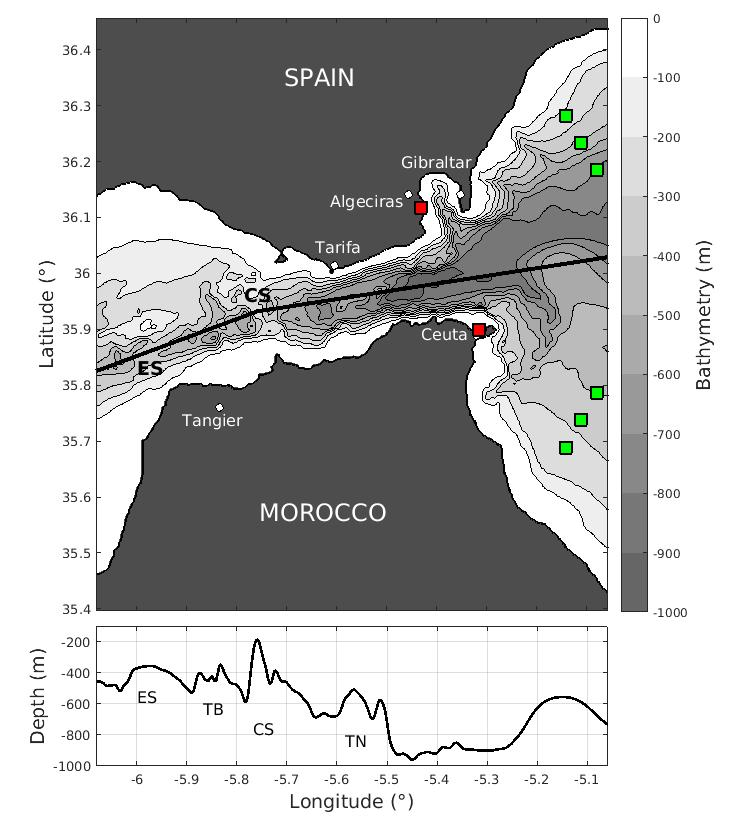
\includegraphics[width=3.77in,height=4.44in]{./media/image1.jpg}
	\end{Center}

%%%%%%%%%%%%%%%%%%%% Figure/Image No: 1 Ends here %%%%%%%%%%%%%%%%%%%%

\caption { Bathymetry and domain extension of R\textsubscript{NBQ} $\&$  R\textsubscript{H}. The black line locate the vertical transect/section on the lower plot. Red squares locate tidal gauges position and green squares locate Xtrack position.}
 \label{Fig1_Lucie}
\end{figure}

\vspace{\baselineskip}
\subsection{Barotropic tides}

\vspace{\baselineskip}
Barotropic tides in the region present an original pattern due to the complex geometry of the strait and its strong dynamics. The tides are typically semi-diurnal, as in the whole Northern Atlantic Ocean, and flowing back and forth zonally at a first glance. The large tidal flows at the Atlantic entrance are strongly reduced in the strait to enter the Mediterranean Sea with typical amplitudes of a few tens of centimeters. The adjustment of the flow imposes complex tidal patterns into the Strait itself making the modelling of barotropic tides in the strait region very challenging. \\
This complexity is circumvented in state-of-the-art barotropic tidal models thanks to the assimilation of altimeter data particularly. But, into the Strait, the lack of data to constrain the cotidal charts makes these global models very precise outside the Strait but less inside. So the forcing they can impose at the boundary of a reduced modelling domain centered on the Strait is generally an important source of error. A huge modelling effort is thus necessary to assess the sensitivity of CROCO to various parameters (bathymetry, open-boundary conditions, forcing atlas...). Additional work (eg. bathymetry, bottom friction, large-scale forcing compatibility, ... ) will be needed to overcome the remaining difficulties.\\
Both configurations (R\textsubscript{NBQ} $\&$  R\textsubscript{H}) run over two spring neap cycles, and the results are compared with available observed data (X-TRACK altimetry and tidal gauges). \par
In Tables \ref{Tab1_Lucie}, \ref{Tab2_Lucie} and \ref{Tab3_Lucie} the observed and simulated amplitudes ($A$) and phases ($G$) are compared for the
main barotropic tidal components (M2, S2, K1, O1). As expected, the simulated amplitudes ($A$) and phases ($G$) of the four tidal components are very similar in the hydrostatic and non-hydrostatic runs.\\

A good agreement between observed and predicted values is found; the maximum differences do not exceed 4.8 cm in amplitude and 11.3° in phase for the semi-diurnal components. The relative errors (dE/A) are significant for the diurnal components (O1, K1), however the amplitudes of these components are quite small in that region.


%%%%%%%%%%%%%%%%%%%% Table No: 2 starts here %%%%%%%%%%%%%%%%%%%%


\begin{table}[!h]
 			\centering
\begin{tabular}{p{0.25in}p{0.31in}p{0.54in}p{0.54in}p{0.54in}p{0.5in}p{0.54in}p{0.54in}p{0.54in}p{0.5in}}
\hline
%row no:1
\multicolumn{2}{|p{0.56in}}{\Centering {\fontsize{11pt}{13.2pt}\selectfont Simulation}} & 
\multicolumn{4}{|p{2.12in}}{\Centering {\fontsize{11pt}{13.2pt}\selectfont R\textsubscript{NBQ}}} & 
\multicolumn{4}{|p{2.12in}|}{\Centering {\fontsize{11pt}{13.2pt}\selectfont R\textsubscript{H}}} \\
\hhline{----------}
%row no:2
\multicolumn{2}{|p{0.56in}}{\cellcolor[HTML]{EFEFEF}} & 
\multicolumn{1}{|p{0.54in}}{\cellcolor[HTML]{EFEFEF}\Centering {\fontsize{11pt}{13.2pt}\selectfont dA (cm)}} & 
\multicolumn{1}{|p{0.54in}}{\cellcolor[HTML]{EFEFEF}\Centering {\fontsize{11pt}{13.2pt}\selectfont dG ($ ^{\circ} $)}} & 
\multicolumn{1}{|p{0.54in}}{\cellcolor[HTML]{EFEFEF}\Centering {\fontsize{11pt}{13.2pt}\selectfont $ \vert\vert dE \vert\vert$  (cm)}} & 
\multicolumn{1}{|p{0.5in}}{\cellcolor[HTML]{EFEFEF}\Centering {\fontsize{11pt}{13.2pt}\selectfont \Tiny{\textbf{$ \vert\vert dE \vert\vert/A$ ($\%$ )}}}} & 
\multicolumn{1}{|p{0.54in}}{\cellcolor[HTML]{EFEFEF}\Centering {\fontsize{11pt}{13.2pt}\selectfont dA (cm)}} & 
\multicolumn{1}{|p{0.54in}}{\cellcolor[HTML]{EFEFEF}\Centering {\fontsize{11pt}{13.2pt}\selectfont dG ($ ^{\circ} $)}} & 
\multicolumn{1}{|p{0.54in}}{\cellcolor[HTML]{EFEFEF}\Centering {\fontsize{11pt}{13.2pt}\selectfont $ \vert\vert dE \vert\vert$ (cm)}} & 
\multicolumn{1}{|p{0.5in}|}{\cellcolor[HTML]{EFEFEF}\Centering {\fontsize{11pt}{13.2pt}\selectfont \Tiny{\textbf{$ \vert\vert dE \vert\vert/A$ ($\%$ )}}}} \\
\hhline{----------}
%row no:3
\multicolumn{1}{|p{0.25in}}{\multirowcell{}{}{\begin{tabular}{p{0.16in}}\Centering {\fontsize{11pt}{13.2pt}\selectfont M2}\\\end{tabular}}} & 
\multicolumn{1}{|p{0.31in}}{\Centering {\fontsize{11pt}{13.2pt}\selectfont North}} & 
\multicolumn{1}{|p{0.54in}}{\Centering {\fontsize{9pt}{10.8pt}\selectfont 4.8+-0.7}} & 
\multicolumn{1}{|p{0.54in}}{\Centering {\fontsize{9pt}{10.8pt}\selectfont 0.7+-3.6}} & 
\multicolumn{1}{|p{0.54in}}{\Centering {\fontsize{9pt}{10.8pt}\selectfont 3.4+-1.2}} & 
\multicolumn{1}{|p{0.5in}}{\Centering {\fontsize{10pt}{12.0pt}\selectfont \textbf{15.3}}} & 
\multicolumn{1}{|p{0.54in}}{\Centering {\fontsize{9pt}{10.8pt}\selectfont 4.8+-0.7}} & 
\multicolumn{1}{|p{0.54in}}{\Centering {\fontsize{9pt}{10.8pt}\selectfont 0.3+-3.6}} & 
\multicolumn{1}{|p{0.54in}}{\Centering {\fontsize{9pt}{10.8pt}\selectfont 3.4+-1.2}} & 
\multicolumn{1}{|p{0.5in}|}{\Centering {\fontsize{10pt}{12.0pt}\selectfont \textbf{15.3}}} \\
\hhline{~---------}
%row no:4
\multicolumn{1}{|p{0.25in}}{} & 
\multicolumn{1}{|p{0.31in}}{\Centering {\fontsize{11pt}{13.2pt}\selectfont South}} & 
\multicolumn{1}{|p{0.54in}}{\Centering {\fontsize{9pt}{10.8pt}\selectfont 4.5+-0.7}} & 
\multicolumn{1}{|p{0.54in}}{\Centering {\fontsize{9pt}{10.8pt}\selectfont -10.6+-4.4}} & 
\multicolumn{1}{|p{0.54in}}{\Centering {\fontsize{9pt}{10.8pt}\selectfont 4.3+-1.4}} & 
\multicolumn{1}{|p{0.5in}}{\Centering {\fontsize{10pt}{12.0pt}\selectfont \textbf{19.5}}} & 
\multicolumn{1}{|p{0.54in}}{\Centering {\fontsize{9pt}{10.8pt}\selectfont 4.4+-0.7}} & 
\multicolumn{1}{|p{0.54in}}{\Centering {\fontsize{9pt}{10.8pt}\selectfont -11.1+-4.4}} & 
\multicolumn{1}{|p{0.54in}}{\Centering {\fontsize{9pt}{10.8pt}\selectfont 4.4+-1.5}} & 
\multicolumn{1}{|p{0.5in}|}{\Centering {\fontsize{10pt}{12.0pt}\selectfont \textbf{19.6}}} \\
\hhline{----------}
%row no:5
\multicolumn{1}{|p{0.25in}}{\multirow{1}{*}{\begin{tabular}{p{0.16in}}\cellcolor[HTML]{EFEFEF}\Centering {\fontsize{11pt}{13.2pt}\selectfont S2}\\\end{tabular}}} & 
\multicolumn{1}{|p{0.31in}}{\cellcolor[HTML]{EFEFEF}\Centering {\fontsize{11pt}{13.2pt}\selectfont North}} & 
\multicolumn{1}{|p{0.54in}}{\cellcolor[HTML]{EFEFEF}\Centering {\fontsize{9pt}{10.8pt}\selectfont 0.1+-2}} & 
\multicolumn{1}{|p{0.54in}}{\cellcolor[HTML]{EFEFEF}\Centering {\fontsize{9pt}{10.8pt}\selectfont 11.3+-16}} & 
\multicolumn{1}{|p{0.54in}}{\cellcolor[HTML]{EFEFEF}\Centering {\fontsize{9pt}{10.8pt}\selectfont 0.9+-2}} & 
\multicolumn{1}{|p{0.5in}}{\cellcolor[HTML]{EFEFEF}\Centering {\fontsize{10pt}{12.0pt}\selectfont \textbf{24}}} & 
\multicolumn{1}{|p{0.54in}}{\cellcolor[HTML]{EFEFEF}\Centering {\fontsize{9pt}{10.8pt}\selectfont 0.2+-1.8}} & 
\multicolumn{1}{|p{0.54in}}{\cellcolor[HTML]{EFEFEF}\Centering {\fontsize{9pt}{10.8pt}\selectfont 11.3+-16}} & 
\multicolumn{1}{|p{0.54in}}{\cellcolor[HTML]{EFEFEF}\Centering {\fontsize{9pt}{10.8pt}\selectfont 0.8+-1.9}} & 
\multicolumn{1}{|p{0.5in}|}{\cellcolor[HTML]{EFEFEF}\Centering {\fontsize{10pt}{12.0pt}\selectfont \textbf{23.5}}} \\
\hhline{~---------}
%row no:6
\multicolumn{1}{|p{0.25in}}{\cellcolor[HTML]{EFEFEF}} & 
\multicolumn{1}{|p{0.31in}}{\cellcolor[HTML]{EFEFEF}\Centering {\fontsize{11pt}{13.2pt}\selectfont South}} & 
\multicolumn{1}{|p{0.54in}}{\cellcolor[HTML]{EFEFEF}\Centering {\fontsize{9pt}{10.8pt}\selectfont 1.2+-0.9}} & 
\multicolumn{1}{|p{0.54in}}{\cellcolor[HTML]{EFEFEF}\Centering {\fontsize{9pt}{10.8pt}\selectfont -5.5+-3}} & 
\multicolumn{1}{|p{0.54in}}{\cellcolor[HTML]{EFEFEF}\Centering {\fontsize{9pt}{10.8pt}\selectfont 1+-0.7}} & 
\multicolumn{1}{|p{0.5in}}{\cellcolor[HTML]{EFEFEF}\Centering {\fontsize{10pt}{12.0pt}\selectfont \textbf{14.1}}} & 
\multicolumn{1}{|p{0.54in}}{\cellcolor[HTML]{EFEFEF}\Centering {\fontsize{9pt}{10.8pt}\selectfont 1.2+1.0}} & 
\multicolumn{1}{|p{0.54in}}{\cellcolor[HTML]{EFEFEF}\Centering {\fontsize{9pt}{10.8pt}\selectfont -6.0+-3}} & 
\multicolumn{1}{|p{0.54in}}{\cellcolor[HTML]{EFEFEF}\Centering {\fontsize{9pt}{10.8pt}\selectfont 1+-0.7}} & 
\multicolumn{1}{|p{0.5in}|}{\cellcolor[HTML]{EFEFEF}\Centering {\fontsize{10pt}{12.0pt}\selectfont \textbf{14.3}}} \\
\hhline{----------}
%row no:7
\multicolumn{1}{|p{0.25in}}{\multirow{1}{*}{\begin{tabular}{p{0.16in}}\Centering {\fontsize{11pt}{13.2pt}\selectfont K1}\\\end{tabular}}} & 
\multicolumn{1}{|p{0.31in}}{\Centering {\fontsize{11pt}{13.2pt}\selectfont North}} & 
\multicolumn{1}{|p{0.54in}}{\Centering {\fontsize{9pt}{10.8pt}\selectfont -0.01+-0.1}} & 
\multicolumn{1}{|p{0.54in}}{\Centering {\fontsize{9pt}{10.8pt}\selectfont 2.2+-1.8}} & 
\multicolumn{1}{|p{0.54in}}{\Centering {\fontsize{9pt}{10.8pt}\selectfont 0.1+-0.7}} & 
\multicolumn{1}{|p{0.5in}}{\Centering {\fontsize{10pt}{12.0pt}\selectfont \textbf{20.4}}} & 
\multicolumn{1}{|p{0.54in}}{\Centering {\fontsize{9pt}{10.8pt}\selectfont -0.02+-1.0}} & 
\multicolumn{1}{|p{0.54in}}{\Centering {\fontsize{9pt}{10.8pt}\selectfont 0.8+-1.1}} & 
\multicolumn{1}{|p{0.54in}}{\Centering {\fontsize{9pt}{10.8pt}\selectfont 0.1+-0.7}} & 
\multicolumn{1}{|p{0.5in}|}{\Centering {\fontsize{10pt}{12.0pt}\selectfont \textbf{21.1}}} \\
\hhline{~---------}
%row no:8
\multicolumn{1}{|p{0.25in}}{} & 
\multicolumn{1}{|p{0.31in}}{\Centering {\fontsize{11pt}{13.2pt}\selectfont South}} & 
\multicolumn{1}{|p{0.54in}}{\Centering {\fontsize{9pt}{10.8pt}\selectfont -1.7+-0.8}} & 
\multicolumn{1}{|p{0.54in}}{\Centering {\fontsize{9pt}{10.8pt}\selectfont 37.8+-2.5}} & 
\multicolumn{1}{|p{0.54in}}{\Centering {\fontsize{9pt}{10.8pt}\selectfont 1.6+-0.5}} & 
\multicolumn{1}{|p{0.5in}}{\Centering {\fontsize{10pt}{12.0pt}\selectfont \textbf{66.5}}} & 
\multicolumn{1}{|p{0.54in}}{\Centering {\fontsize{9pt}{10.8pt}\selectfont -1.5+-0.8}} & 
\multicolumn{1}{|p{0.54in}}{\Centering {\fontsize{9pt}{10.8pt}\selectfont 37.8+-2.3}} & 
\multicolumn{1}{|p{0.54in}}{\Centering {\fontsize{9pt}{10.8pt}\selectfont 1.6+-0.5}} & 
\multicolumn{1}{|p{0.5in}|}{\Centering {\fontsize{10pt}{12.0pt}\selectfont \textbf{65.4}}} \\
\hhline{----------}
%row no:9
\multicolumn{1}{|p{0.25in}}{\multirow{1}{*}{\begin{tabular}{p{0.16in}}\cellcolor[HTML]{EFEFEF}\Centering {\fontsize{11pt}{13.2pt}\selectfont O1}\\\end{tabular}}} & 
\multicolumn{1}{|p{0.31in}}{\cellcolor[HTML]{EFEFEF}\Centering {\fontsize{11pt}{13.2pt}\selectfont North}} & 
\multicolumn{1}{|p{0.54in}}{\cellcolor[HTML]{EFEFEF}\Centering {\fontsize{9pt}{10.8pt}\selectfont -0.8+-0.6}} & 
\multicolumn{1}{|p{0.54in}}{\cellcolor[HTML]{EFEFEF}\Centering {\fontsize{9pt}{10.8pt}\selectfont -10.7$ \pm $ 13.6}} & 
\multicolumn{1}{|p{0.54in}}{\cellcolor[HTML]{EFEFEF}\Centering {\fontsize{9pt}{10.8pt}\selectfont 0.7+-0.5}} & 
\multicolumn{1}{|p{0.5in}}{\cellcolor[HTML]{EFEFEF}\Centering {\fontsize{10pt}{12.0pt}\selectfont \textbf{46.6}}} & 
\multicolumn{1}{|p{0.54in}}{\cellcolor[HTML]{EFEFEF}\Centering {\fontsize{9pt}{10.8pt}\selectfont -1+-0.6}} & 
\multicolumn{1}{|p{0.54in}}{\cellcolor[HTML]{EFEFEF}\Centering {\fontsize{9pt}{10.8pt}\selectfont -8.1$ \pm $ 13.0}} & 
\multicolumn{1}{|p{0.54in}}{\cellcolor[HTML]{EFEFEF}\Centering {\fontsize{9pt}{10.8pt}\selectfont 0.8+-0.5}} & 
\multicolumn{1}{|p{0.5in}|}{\cellcolor[HTML]{EFEFEF}\Centering {\fontsize{10pt}{12.0pt}\selectfont \textbf{48.8}}} \\
\hhline{~---------}
%row no:10
\multicolumn{1}{|p{0.25in}}{\cellcolor[HTML]{EFEFEF}} & 
\multicolumn{1}{|p{0.31in}}{\cellcolor[HTML]{EFEFEF}\Centering {\fontsize{11pt}{13.2pt}\selectfont South}} & 
\multicolumn{1}{|p{0.54in}}{\cellcolor[HTML]{EFEFEF}\Centering {\fontsize{10pt}{12.0pt}\selectfont 0.2+-0.5}} & 
\multicolumn{1}{|p{0.54in}}{\cellcolor[HTML]{EFEFEF}\Centering {\fontsize{10pt}{12.0pt}\selectfont -8.5+-18.5}} & 
\multicolumn{1}{|p{0.54in}}{\cellcolor[HTML]{EFEFEF}\Centering {\fontsize{10pt}{12.0pt}\selectfont 0.2+-0.7}} & 
\multicolumn{1}{|p{0.5in}}{\cellcolor[HTML]{EFEFEF}\Centering {\fontsize{10pt}{12.0pt}\selectfont \textbf{25.6}}} & 
\multicolumn{1}{|p{0.54in}}{\cellcolor[HTML]{EFEFEF}\Centering {\fontsize{10pt}{12.0pt}\selectfont 0.09+-0.5}} & 
\multicolumn{1}{|p{0.54in}}{\cellcolor[HTML]{EFEFEF}\Centering {\fontsize{10pt}{12.0pt}\selectfont -5.7+-18.6}} & 
\multicolumn{1}{|p{0.54in}}{\cellcolor[HTML]{EFEFEF}\Centering {\fontsize{10pt}{12.0pt}\selectfont 0.1+-0.7}} & 
\multicolumn{1}{|p{0.5in}|}{\cellcolor[HTML]{EFEFEF}\Centering {\fontsize{10pt}{12.0pt}\selectfont \textbf{25.3}}} \\
\hhline{----------}

\end{tabular}


%%%%%%%%%%%%%%%%%%%% Table No: 2 ends here %%%%%%%%%%%%%%%%%%%%
\caption{Model performance statistics for the main barotropic tidal components (M2, S2, K1, O1) in \textbf{R\textsubscript{NBQ}}\textsubscript{ }$\&$ \textbf{ R\textsubscript{H}} in comparison to X-TRACK altimetry. dA = mean amplitude biais; dG = mean phase bias; $ \vert $ $ \vert $ dE$ \vert $ $ \vert $ \ = mean combined bias;  $ \vert $ $ \vert $ dE$ \vert $ $ \vert $ /A = mean relative bias.}
\label{Tab2_Lucie}

 \end{table}

%%%%%%%%%%%%%%%%%%%% Table No: 3 starts here %%%%%%%%%%%%%%%%%%%%


\begin{table}[!h]
 			\centering
\begin{tabular}{p{0.25in}p{0.4in}p{0.47in}p{0.6in}p{0.5in}p{0.49in}p{0.5in}p{0.5in}p{0.5in}p{0.5in}}
%\begin{tabular}{p{0.23in}p{0.4in}p{0.47in}p{0.61in}p{0.61in}p{0.49in}p{0.69in}p{0.59in}p{0.59in}p{0.69in}}
\hline
%row no:1
\multicolumn{2}{|p{0.65in}}{\Centering {\fontsize{11pt}{13.2pt}\selectfont Simulation}} & 
\multicolumn{4}{|p{2.06in}}{\Centering {\fontsize{11pt}{13.2pt}\selectfont Forcing (MITgcm)}} & 
\multicolumn{4}{|p{2.0in}|}{\Centering {\fontsize{11pt}{13.2pt}\selectfont TPX08}} \\
\hhline{----------}
%row no:2
\multicolumn{2}{|p{0.65in}}{\cellcolor[HTML]{EFEFEF}} & 
\multicolumn{1}{|p{0.47in}}{\cellcolor[HTML]{EFEFEF}\Centering {\fontsize{11pt}{13.2pt}\selectfont dA (cm)}} & 
\multicolumn{1}{|p{0.61in}}{\cellcolor[HTML]{EFEFEF}\Centering {\fontsize{11pt}{13.2pt}\selectfont dG ($ ^{\circ} $)}} & 
\multicolumn{1}{|p{0.61in}}{\cellcolor[HTML]{EFEFEF}\Centering {\fontsize{11pt}{13.2pt}\selectfont $ \vert\vert dE \vert\vert $  (cm)}} & 
\multicolumn{1}{|p{0.4in}}{\cellcolor[HTML]{EFEFEF}\Centering {\fontsize{11pt}{13.2pt}\selectfont \Tiny{\textbf{$ \vert\vert dE\vert\vert/A$ ($\%$)}}}} & 
\multicolumn{1}{|p{0.55in}}{\cellcolor[HTML]{EFEFEF}\Centering {\fontsize{11pt}{13.2pt}\selectfont dA (cm)}} & 
\multicolumn{1}{|p{0.5in}}{\cellcolor[HTML]{EFEFEF}\Centering {\fontsize{11pt}{13.2pt}\selectfont dG ($ ^{\circ} $)}} & 
\multicolumn{1}{|p{0.5in}}{\cellcolor[HTML]{EFEFEF}\Centering {\fontsize{11pt}{13.2pt}\selectfont $\vert\vert dE\vert\vert$ (cm)}} & 
\multicolumn{1}{|p{0.5in}|}{\cellcolor[HTML]{EFEFEF}\Centering {\fontsize{11pt}{13.2pt}\selectfont \Tiny{\textbf{$ \vert\vert dE \vert\vert/A$ ($\%$)}}}} \\
\hhline{----------}
%row no:3
\multicolumn{1}{|p{0.25in}}{\multirowcell{}{}{\begin{tabular}{p{0.01in}}\Centering {\fontsize{11pt}{13.2pt}\selectfont M2}\\\end{tabular}}} & 
\multicolumn{1}{|p{0.4in}}{\Centering {\fontsize{11pt}{13.2pt}\selectfont North}} & 
\multicolumn{1}{|p{0.47in}}{\Centering {\fontsize{10pt}{12.0pt}\selectfont 4.8 $ \pm $ 0.6}} & 
\multicolumn{1}{|p{0.61in}}{\Centering {\fontsize{10pt}{12.0pt}\selectfont 9.1 $ \pm $ 3.3}} & 
\multicolumn{1}{|p{0.61in}}{\Centering {\fontsize{10pt}{12.0pt}\selectfont 4.2$ \pm $ 1.1}} & 
\multicolumn{1}{|p{0.49in}}{\Centering {\fontsize{10pt}{12.0pt}\selectfont \textbf{18.5}}} & 
\multicolumn{1}{|p{0.5in}}{\Centering {\fontsize{10pt}{12.0pt}\selectfont 0.9 $ \pm $ 0.4}} & 
\multicolumn{1}{|p{0.5in}}{\Centering {\fontsize{10pt}{12.0pt}\selectfont 0.7$ \pm $ 3.6}} & 
\multicolumn{1}{|p{0.5in}}{\Centering {\fontsize{10pt}{12.0pt}\selectfont 0.6$ \pm $ 1.2}} & 
\multicolumn{1}{|p{0.5in}|}{\Centering {\fontsize{10pt}{12.0pt}\selectfont \textbf{4.8}}} \\
\hhline{~---------}
%row no:4
\multicolumn{1}{|p{0.25in}}{} & 
\multicolumn{1}{|p{0.4in}}{\Centering {\fontsize{11pt}{13.2pt}\selectfont South}} & 
\multicolumn{1}{|p{0.47in}}{\Centering {\fontsize{10pt}{12.0pt}\selectfont 5.6$ \pm $ 0.7}} & 
\multicolumn{1}{|p{0.61in}}{\Centering {\fontsize{10pt}{12.0pt}\selectfont 0.5$ \pm $ 4.7}} & 
\multicolumn{1}{|p{0.61in}}{\Centering {\fontsize{10pt}{12.0pt}\selectfont 3.9$ \pm $ 1.5}} & 
\multicolumn{1}{|p{0.49in}}{\Centering {\fontsize{10pt}{12.0pt}\selectfont \textbf{19.0}}} & 
\multicolumn{1}{|p{0.5in}}{\Centering {\fontsize{10pt}{12.0pt}\selectfont 0.3$ \pm $ 0.9}} & 
\multicolumn{1}{|p{0.5in}}{\Centering {\fontsize{10pt}{12.0pt}\selectfont -3.6$ \pm $ 4.5}} & 
\multicolumn{1}{|p{0.5in}}{\Centering {\fontsize{10pt}{12.0pt}\selectfont 1.2$ \pm $ 1.5}} & 
\multicolumn{1}{|p{0.5in}|}{\Centering {\fontsize{10pt}{12.0pt}\selectfont \textbf{6.1}}} \\
\hhline{----------}
%row no:5
\multicolumn{1}{|p{0.25in}}{\multirow{1}{*}{\begin{tabular}{p{0.01in}}\cellcolor[HTML]{EFEFEF}\Centering {\fontsize{11pt}{13.2pt}\selectfont S2}\\\end{tabular}}} & 
\multicolumn{1}{|p{0.4in}}{\cellcolor[HTML]{EFEFEF}\Centering {\fontsize{11pt}{13.2pt}\selectfont North}} & 
\multicolumn{1}{|p{0.47in}}{\Centering {\fontsize{10pt}{12.0pt}\selectfont 0.3$ \pm $ 1.8}} & 
\multicolumn{1}{|p{0.61in}}{\Centering {\fontsize{10pt}{12.0pt}\selectfont 17.5$ \pm $ 15.4}} & 
\multicolumn{1}{|p{0.61in}}{\Centering {\fontsize{10pt}{12.0pt}\selectfont 1.4$ \pm $ 1.9}} & 
\multicolumn{1}{|p{0.49in}}{\cellcolor[HTML]{EFEFEF}\Centering {\fontsize{10pt}{12.0pt}\selectfont \textbf{27.5}}} & 
\multicolumn{1}{|p{0.5in}}{\Centering {\fontsize{10pt}{12.0pt}\selectfont -1.0$ \pm $ 1.8}} & 
\multicolumn{1}{|p{0.5in}}{\Centering {\fontsize{10pt}{12.0pt}\selectfont 12.3$ \pm $ 15.4}} & 
\multicolumn{1}{|p{0.5in}}{\Centering {\fontsize{10pt}{12.0pt}\selectfont 1.3$ \pm $ 1.9}} & 
\multicolumn{1}{|p{0.5in}|}{\cellcolor[HTML]{EFEFEF}\Centering {\fontsize{10pt}{12.0pt}\selectfont \textbf{19.4}}} \\
\hhline{~---------}
%row no:6
\multicolumn{1}{|p{0.25in}}{\cellcolor[HTML]{EFEFEF}} & 
\multicolumn{1}{|p{0.4in}}{\cellcolor[HTML]{EFEFEF}\Centering {\fontsize{11pt}{13.2pt}\selectfont South}} & 
\multicolumn{1}{|p{0.47in}}{\Centering {\fontsize{10pt}{12.0pt}\selectfont -1.2$ \pm $ 0.1}} & 
\multicolumn{1}{|p{0.61in}}{\Centering {\fontsize{10pt}{12.0pt}\selectfont 21.1$ \pm $ 10.5}} & 
\multicolumn{1}{|p{0.61in}}{\Centering {\fontsize{10pt}{12.0pt}\selectfont 1.0$ \pm $ 0.6}} & 
\multicolumn{1}{|p{0.49in}}{\cellcolor[HTML]{EFEFEF}\Centering {\fontsize{10pt}{12.0pt}\selectfont \textbf{13.6}}} & 
\multicolumn{1}{|p{0.5in}}{\Centering {\fontsize{10pt}{12.0pt}\selectfont -0.2$ \pm $ 1.0}} & 
\multicolumn{1}{|p{0.5in}}{\Centering {\fontsize{10pt}{12.0pt}\selectfont -3.9$ \pm $ 2.4}} & 
\multicolumn{1}{|p{0.5in}}{\Centering {\fontsize{10pt}{12.0pt}\selectfont 0.4$ \pm $ 0.8}} & 
\multicolumn{1}{|p{0.5in}|}{\cellcolor[HTML]{EFEFEF}\Centering {\fontsize{10pt}{12.0pt}\selectfont \textbf{9.2}}} \\
\hhline{----------}
%row no:7
\multicolumn{1}{|p{0.25in}}{\multirow{1}{*}{\begin{tabular}{p{0.01in}}\Centering {\fontsize{11pt}{13.2pt}\selectfont K1}\\\end{tabular}}} & 
\multicolumn{1}{|p{0.4in}}{\Centering {\fontsize{11pt}{13.2pt}\selectfont North}} & 
\multicolumn{1}{|p{0.47in}}{\Centering {\fontsize{10pt}{12.0pt}\selectfont 0.4 $ \pm $ 1.0}} & 
\multicolumn{1}{|p{0.61in}}{\Centering {\fontsize{10pt}{12.0pt}\selectfont 8.7 $ \pm $ 1.3}} & 
\multicolumn{1}{|p{0.61in}}{\Centering {\fontsize{10pt}{12.0pt}\selectfont 0.5$ \pm $ 0.7}} & 
\multicolumn{1}{|p{0.49in}}{\Centering {\fontsize{10pt}{12.0pt}\selectfont \textbf{25.9}}} & 
\multicolumn{1}{|p{0.5in}}{\Centering {\fontsize{10pt}{12.0pt}\selectfont 0.5 $ \pm $ 0.9}} & 
\multicolumn{1}{|p{0.5in}}{\Centering {\fontsize{10pt}{12.0pt}\selectfont 14.0 $ \pm $ 2.6}} & 
\multicolumn{1}{|p{0.5in}}{\Centering {\fontsize{10pt}{12.0pt}\selectfont 0.7$ \pm $ 0.7}} & 
\multicolumn{1}{|p{0.5in}|}{\Centering {\fontsize{10pt}{12.0pt}\selectfont \textbf{28.7}}} \\
\hhline{~---------}
%row no:8
\multicolumn{1}{|p{0.25in}}{} & 
\multicolumn{1}{|p{0.4in}}{\Centering {\fontsize{11pt}{13.2pt}\selectfont South}} & 
\multicolumn{1}{|p{0.47in}}{\Centering {\fontsize{10pt}{12.0pt}\selectfont -1.1$ \pm $ 0.8}} & 
\multicolumn{1}{|p{0.61in}}{\Centering {\fontsize{10pt}{12.0pt}\selectfont 44.0$ \pm $ 2.4}} & 
\multicolumn{1}{|p{0.61in}}{\Centering {\fontsize{10pt}{12.0pt}\selectfont 1.4$ \pm $ 0.6}} & 
\multicolumn{1}{|p{0.49in}}{\Centering {\fontsize{10pt}{12.0pt}\selectfont \textbf{66.4}}} & 
\multicolumn{1}{|p{0.5in}}{\Centering {\fontsize{10pt}{12.0pt}\selectfont -1.7$ \pm $ 0.8}} & 
\multicolumn{1}{|p{0.5in}}{\Centering {\fontsize{10pt}{12.0pt}\selectfont 59.8$ \pm $ 3.2}} & 
\multicolumn{1}{|p{0.5in}}{\Centering {\fontsize{10pt}{12.0pt}\selectfont 2.2$ \pm $ 0.5}} & 
\multicolumn{1}{|p{0.5in}|}{\Centering {\fontsize{10pt}{12.0pt}\selectfont \textbf{84.4}}} \\
\hhline{----------}
%row no:9
\multicolumn{1}{|p{0.25in}}{\multirow{1}{*}{\begin{tabular}{p{0.01in}}\cellcolor[HTML]{EFEFEF}\Centering {\fontsize{11pt}{13.2pt}\selectfont O1}\\\end{tabular}}} & 
\multicolumn{1}{|p{0.4in}}{\cellcolor[HTML]{EFEFEF}\Centering {\fontsize{11pt}{13.2pt}\selectfont North}} & 
\multicolumn{1}{|p{0.47in}}{\Centering {\fontsize{10pt}{12.0pt}\selectfont -0.2$ \pm $ 0.5}} & 
\multicolumn{1}{|p{0.61in}}{\Centering {\fontsize{10pt}{12.0pt}\selectfont -15.8$ \pm $ 13}} & 
\multicolumn{1}{|p{0.61in}}{\Centering {\fontsize{10pt}{12.0pt}\selectfont 0.4$ \pm $ 0.5}} & 
\multicolumn{1}{|p{0.49in}}{\cellcolor[HTML]{EFEFEF}\Centering {\fontsize{10pt}{12.0pt}\selectfont \textbf{35.2}}} & 
\multicolumn{1}{|p{0.5in}}{\Centering {\fontsize{10pt}{12.0pt}\selectfont 0.01$ \pm $ 0.5}} & 
\multicolumn{1}{|p{0.5in}}{\Centering {\fontsize{10pt}{12.0pt}\selectfont -3.1$ \pm $ 14.1}} & 
\multicolumn{1}{|p{0.5in}}{\Centering {\fontsize{10pt}{12.0pt}\selectfont 0.1$ \pm $ 0.4}} & 
\multicolumn{1}{|p{0.5in}|}{\cellcolor[HTML]{EFEFEF}\Centering {\fontsize{10pt}{12.0pt}\selectfont \textbf{29.1}}} \\
\hhline{~---------}
%row no:10
\multicolumn{1}{|p{0.25in}}{\cellcolor[HTML]{EFEFEF}} & 
\multicolumn{1}{|p{0.4in}}{\cellcolor[HTML]{EFEFEF}\Centering {\fontsize{11pt}{13.2pt}\selectfont South}} & 
\multicolumn{1}{|p{0.47in}}{\Centering {\fontsize{10pt}{12.0pt}\selectfont 0.7$ \pm $ 0.4}} & 
\multicolumn{1}{|p{0.61in}}{\Centering {\fontsize{10pt}{12.0pt}\selectfont -28.3$ \pm $ 23}} & 
\multicolumn{1}{|p{0.61in}}{\Centering {\fontsize{10pt}{12.0pt}\selectfont 0.8$ \pm $ 0.7}} & 
\multicolumn{1}{|p{0.49in}}{\cellcolor[HTML]{EFEFEF}\Centering {\fontsize{10pt}{12.0pt}\selectfont \textbf{44.3}}} & 
\multicolumn{1}{|p{0.5in}}{\Centering {\fontsize{10pt}{12.0pt}\selectfont 1.1$ \pm $ 0.4}} & 
\multicolumn{1}{|p{0.5in}}{\Centering {\fontsize{10pt}{12.0pt}\selectfont 30.7$ \pm $ 16.5}} & 
\multicolumn{1}{|p{0.5in}}{\Centering {\fontsize{10pt}{12.0pt}\selectfont 1.0$ \pm $ 0.6}} & 
\multicolumn{1}{|p{0.5in}|}{\cellcolor[HTML]{EFEFEF}\Centering {\fontsize{10pt}{12.0pt}\selectfont \textbf{53.5}}} \\
\hhline{----------}

\end{tabular}

\caption{Model performance statistics for the main barotropic tidal components (M2, S2, K1, O1) in the forcing simulation and the state-of-the-art data-assimilated global tidal model TPX08 from OSU  in comparison to X-TRACK altimetry. dA = mean amplitude biais; dG = mean phase bias; $ \vert $ $ \vert $ dE$ \vert $ $ \vert $ \ = mean combined bias;  $ \vert $ $ \vert $ dE$ \vert $ $ \vert $ /A = mean relative bias.}
\label{Tab3_Lucie}
 \end{table}
 
%%%%%%%%%%%%%%%%%%%% Table No: 3 ends here %%%%%%%%%%%%%%%%%%%%



%%%%%%%%%%%%%%%%%%%% Table No: 4 starts here %%%%%%%%%%%%%%%%%%%%


\begin{table}[!h]
 			\centering
\begin{tabular}{p{0.69in}p{0.58in}p{0.58in}p{0.58in}p{0.42in}p{0.54in}p{0.54in}p{0.54in}p{0.5in}}
\hline
%row no:1
\multicolumn{1}{|p{0.69in}}{\Centering {\fontsize{11pt}{13.2pt}\selectfont Simulation}} & 
\multicolumn{4}{|p{2.12in}}{\Centering {\fontsize{11pt}{13.2pt}\selectfont R\textsubscript{NBQ}}} & 
\multicolumn{4}{|p{2.12in}|}{\Centering {\fontsize{11pt}{13.2pt}\selectfont Forcing (MITgcm)}} \\
\hhline{---------}
%row no:2
\multicolumn{1}{|p{0.69in}}{} & 
\multicolumn{1}{|p{0.58in}}{\Centering {\fontsize{11pt}{13.2pt}\selectfont dA (cm)}} & 
\multicolumn{1}{|p{0.58in}}{\Centering {\fontsize{11pt}{13.2pt}\selectfont dG ($ ^{\circ} $)}} & 
\multicolumn{1}{|p{0.58in}}{\Centering {\fontsize{11pt}{13.2pt}\selectfont $ \vert\vert dE \vert\vert$  (cm)}} & 
\multicolumn{1}{|p{0.42in}}{\Centering {\fontsize{11pt}{13.2pt}\selectfont \Tiny{\textbf{$ \vert\vert dE \vert\vert/A$ ($\%$)}}}} & 
\multicolumn{1}{|p{0.54in}}{\Centering {\fontsize{11pt}{13.2pt}\selectfont dA (cm)}} & 
\multicolumn{1}{|p{0.54in}}{\Centering {\fontsize{11pt}{13.2pt}\selectfont dG ($ ^{\circ} $)}} & 
\multicolumn{1}{|p{0.54in}}{\Centering {\fontsize{11pt}{13.2pt}\selectfont $ \vert\vert dE\vert\vert $ (cm)}} & 
\multicolumn{1}{|p{0.5in}|}{\Centering {\fontsize{11pt}{13.2pt}\selectfont \Tiny{\textbf{$ \vert\vert dE \vert\vert/A$ ($\%$ )}}}} \\
\hhline{---------}
%row no:3
\multicolumn{1}{|p{0.69in}}{\Centering {\fontsize{11pt}{13.2pt}\selectfont M2}} & 
\multicolumn{1}{|p{0.58in}}{\Centering {\fontsize{10pt}{12.0pt}\selectfont 3.9 $ \pm $ 0.4}} & 
\multicolumn{1}{|p{0.58in}}{\Centering {\fontsize{10pt}{12.0pt}\selectfont -1.6 $ \pm $ 1.5}} & 
\multicolumn{1}{|p{0.58in}}{\Centering {\fontsize{10pt}{12.0pt}\selectfont 2.8$ \pm $ 0.5}} & 
\multicolumn{1}{|p{0.42in}}{\Centering {\fontsize{10pt}{12.0pt}\selectfont \textbf{9.8}}} & 
\multicolumn{1}{|p{0.54in}}{\Centering {\fontsize{10pt}{12.0pt}\selectfont -4.5$ \pm $ 0.5}} & 
\multicolumn{1}{|p{0.54in}}{\Centering {\fontsize{10pt}{12.0pt}\selectfont 4.6$ \pm $ 1.0}} & 
\multicolumn{1}{|p{0.54in}}{\Centering {\fontsize{10pt}{12.0pt}\selectfont 3.6$ \pm $ 0.5}} & 
\multicolumn{1}{|p{0.5in}|}{\Centering {\fontsize{10pt}{12.0pt}\selectfont \textbf{12.7}}} \\
\hhline{---------}
%row no:4
\multicolumn{1}{|p{0.69in}}{\Centering {\fontsize{11pt}{13.2pt}\selectfont S2}} & 
\multicolumn{1}{|p{0.58in}}{\Centering {\fontsize{10pt}{12.0pt}\selectfont 0.6$ \pm $ 0.3}} & 
\multicolumn{1}{|p{0.58in}}{\Centering {\fontsize{10pt}{12.0pt}\selectfont -1.5$ \pm $ 0.9}} & 
\multicolumn{1}{|p{0.58in}}{\Centering {\fontsize{10pt}{12.0pt}\selectfont 0.5$ \pm $ 0.2}} & 
\multicolumn{1}{|p{0.42in}}{\Centering {\fontsize{10pt}{12.0pt}\selectfont \textbf{4.7}}} & 
\multicolumn{1}{|p{0.54in}}{\Centering {\fontsize{10pt}{12.0pt}\selectfont 1.1$ \pm $ 0.3}} & 
\multicolumn{1}{|p{0.54in}}{\Centering {\fontsize{10pt}{12.0pt}\selectfont 2.8$ \pm $ 0.6}} & 
\multicolumn{1}{|p{0.54in}}{\Centering {\fontsize{10pt}{12.0pt}\selectfont 0.9$ \pm $ 0.2}} & 
\multicolumn{1}{|p{0.5in}|}{\Centering {\fontsize{10pt}{12.0pt}\selectfont \textbf{8.4}}} \\
\hhline{---------}
%row no:5
\multicolumn{1}{|p{0.69in}}{\Centering {\fontsize{11pt}{13.2pt}\selectfont K1}} & 
\multicolumn{1}{|p{0.58in}}{\Centering {\fontsize{10pt}{12.0pt}\selectfont -1.3$ \pm $ 0.6}} & 
\multicolumn{1}{|p{0.58in}}{\Centering {\fontsize{10pt}{12.0pt}\selectfont -5.1$ \pm $ 0.1}} & 
\multicolumn{1}{|p{0.58in}}{\Centering {\fontsize{10pt}{12.0pt}\selectfont 0.9$ \pm $ 0.4}} & 
\multicolumn{1}{|p{0.42in}}{\Centering {\fontsize{10pt}{12.0pt}\selectfont \textbf{24.2}}} & 
\multicolumn{1}{|p{0.54in}}{\Centering {\fontsize{10pt}{12.0pt}\selectfont -1.0$ \pm $ 0.3}} & 
\multicolumn{1}{|p{0.54in}}{\Centering {\fontsize{10pt}{12.0pt}\selectfont 0.2$ \pm $ 0.0}} & 
\multicolumn{1}{|p{0.54in}}{\Centering {\fontsize{10pt}{12.0pt}\selectfont 0.7$ \pm $ 0.2}} & 
\multicolumn{1}{|p{0.5in}|}{\Centering {\fontsize{10pt}{12.0pt}\selectfont \textbf{20.6}}} \\
\hhline{---------}
%row no:6
\multicolumn{1}{|p{0.69in}}{\Centering {\fontsize{11pt}{13.2pt}\selectfont O1}} & 
\multicolumn{1}{|p{0.58in}}{\Centering {\fontsize{10pt}{12.0pt}\selectfont -1.2$ \pm $ 0.1}} & 
\multicolumn{1}{|p{0.58in}}{\Centering {\fontsize{10pt}{12.0pt}\selectfont 21.1$ \pm $ 10.5}} & 
\multicolumn{1}{|p{0.58in}}{\Centering {\fontsize{10pt}{12.0pt}\selectfont 1.0$ \pm $ 0.6}} & 
\multicolumn{1}{|p{0.42in}}{\Centering {\fontsize{10pt}{12.0pt}\selectfont \textbf{47.5}}} & 
\multicolumn{1}{|p{0.54in}}{\Centering {\fontsize{10pt}{12.0pt}\selectfont -0.7$ \pm $ 0.6}} & 
\multicolumn{1}{|p{0.54in}}{\Centering {\fontsize{10pt}{12.0pt}\selectfont 16.6$ \pm $ 8.1}} & 
\multicolumn{1}{|p{0.54in}}{\Centering {\fontsize{10pt}{12.0pt}\selectfont 0.6$ \pm $ 0.4}} & 
\multicolumn{1}{|p{0.5in}|}{\Centering {\fontsize{10pt}{12.0pt}\selectfont \textbf{33.5}}} \\
\hhline{---------}

\end{tabular}

%%%%%%%%%%%%%%%%%%%% Table No: 4 ends here %%%%%%%%%%%%%%%%%%%%

\caption{Model performance statistics for the main barotropic tidal components (M2, S2, K1, O1) in \textbf{R\textsubscript{NBQ}} and the forcing simulation in comparison to tidal gauges. dA = mean amplitude biais; dG = mean phase bias; $ \vert $ $ \vert $ dE$ \vert $ $ \vert $ \ = mean combined bias;  $ \vert $ $ \vert $ dE$ \vert $ $ \vert $ /A = mean relative bias.}
\label{Tab4_Lucie}

 \end{table}

\vspace{\baselineskip}
\subsection{Internal fine-scale processes }

\vspace{\baselineskip}
We now focus on internal fine-scale processes generated by tidal flows. In Gibraltar-strait area, such processes are subject to a strong neap-spring tidal variability. Hence, to study their dynamic, three regimes of tidal forcing during the modelled time period (Figure \ref{Fig3_Lucie}) can be distinguished:\par

\begin{itemize}
	\item a week tidal forcing when the minimal barotropic\ velocity above CS crest  during the tidal outflow is superior to -0.5 m/s (green curve)\par

	\item a moderate tidal forcing when the minimal barotropic\ velocity above CS crest  during the tidal outflow is inferior to -0.5 m/s and superior to -1.5 m/s (blue curve)\par

	\item a strong tidal forcing when the minimal barotropic\ velocity above CS crest  during the tidal outflow is inferior to -1.5 m/s (red curve)
\end{itemize}
During the simulated time-period (1 month), the moderate tidal forcing is the dominant regime.\\
\vspace{\baselineskip}


%%%%%%%%%%%%%%%%%%%% Figure/Image No: 2 starts here %%%%%%%%%%%%%%%%%%%%

\begin{figure}[!h]
	\begin{Center}
		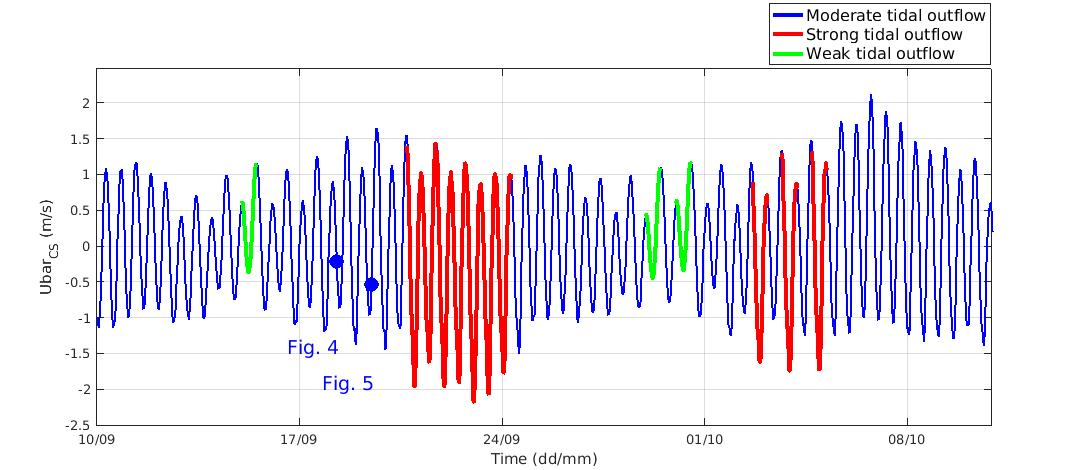
\includegraphics[width=6.3in,height=2.75in]{./media/image2.jpg}
	\end{Center}

%%%%%%%%%%%%%%%%%%%% Figure/Image No: 2 Ends here %%%%%%%%%%%%%%%%%%%%

\caption{Barotropic velocity above CS crest. The colored curves differentiate the three different tidal regimes : green curves - weak tidal forcing, blue curves - moderate tidal forcing and red curves - strong tidal forcing. The circle markers indicate the acquisition date of the high-resolution satellite images on\  figures \ref{Fig4_Lucie} and \ref{Fig5_Lucie}.}
\label{Fig2_Lucie}
\end{figure}

\subsubsection{Comparison to high-resolution satellite images}

\vspace{\baselineskip}
An effective procedure to trace the evolution of the internal or baroclinic field consists of monitoring the spatial gradient of surface velocity. The superposition of baroclinic and barotropic currents gives rise to areas of strong horizontal convergence/divergence of the flow characterized by short-scale surface roughness which can be captured by SARs [Alpers, 1985] and MSI- Multispectral Imager. This allows the identification of baroclinic structures such as internal hydraulic jumps or internal propagating internal waves through the observation of the ocean surface. \par


\vspace{\baselineskip}
Multiple SAR and RGB images have been acquired from Sentinel-1 and Sentinel-2 satellites during the modelled time period (10/09/2017 - 10/10/2017). We focus on two particular satellite images acquired both in moderate regime but at different phases of the tidal cycle: \par

- a SAR image acquired on the 18/09/2017 – 06:27:42\textit{\  }at the end of the tidal cycle\par

- a RGB image acquired \textit{ }the 19/09/2017 – 11:18:00 just after the tidal maximal outflow. \par


\vspace{\baselineskip}
The SAR image was taken at the end of a moderate tidal cycle when the well-known train of ISWs propagating eastward reaches the bay of Gibraltar (Figure \ref{Fig4_Lucie} - Left panel). The train of ISWs on the SAR image is composed at least of 4 distinct solitary waves. On this particular SAR image, a second feature is identifiable as a westward propagating internal wave in Tangier Bassin. The origin of these westward propagating internal waves will be discuss in section 2.4.3.\par

\vspace{\baselineskip}
In R\textsubscript{NBQ}, the train is composed solely of one or two solitary waves (figure \ref{Fig4_Lucie} - Right) however it reaches the bay of Gilbratar at approximately the same moment. Hence, even if the number of solitary waves in the train is underestimated in R\textsubscript{NBQ}, the propagation speed of the train seems to be well represented. Moreover, the westward propagating internal wave observed in Tangier Bassin are also quite well represented in R\textsubscript{NBQ} (location, orientation, shape). The resolution of the SAR image is 10 m, compared with a resolution of 220 m for R\textsubscript{NBQ}. The resolution of R\textsubscript{NBQ} seems therefore insufficient to represent explicitly the smallest solitary waves of the train. 
\par

%%%%%%%%%%%%%%%%%%%% Figure/Image No: 3 starts here %%%%%%%%%%%%%%%%%%%%

\begin{figure}[!h]
	\begin{Center}
		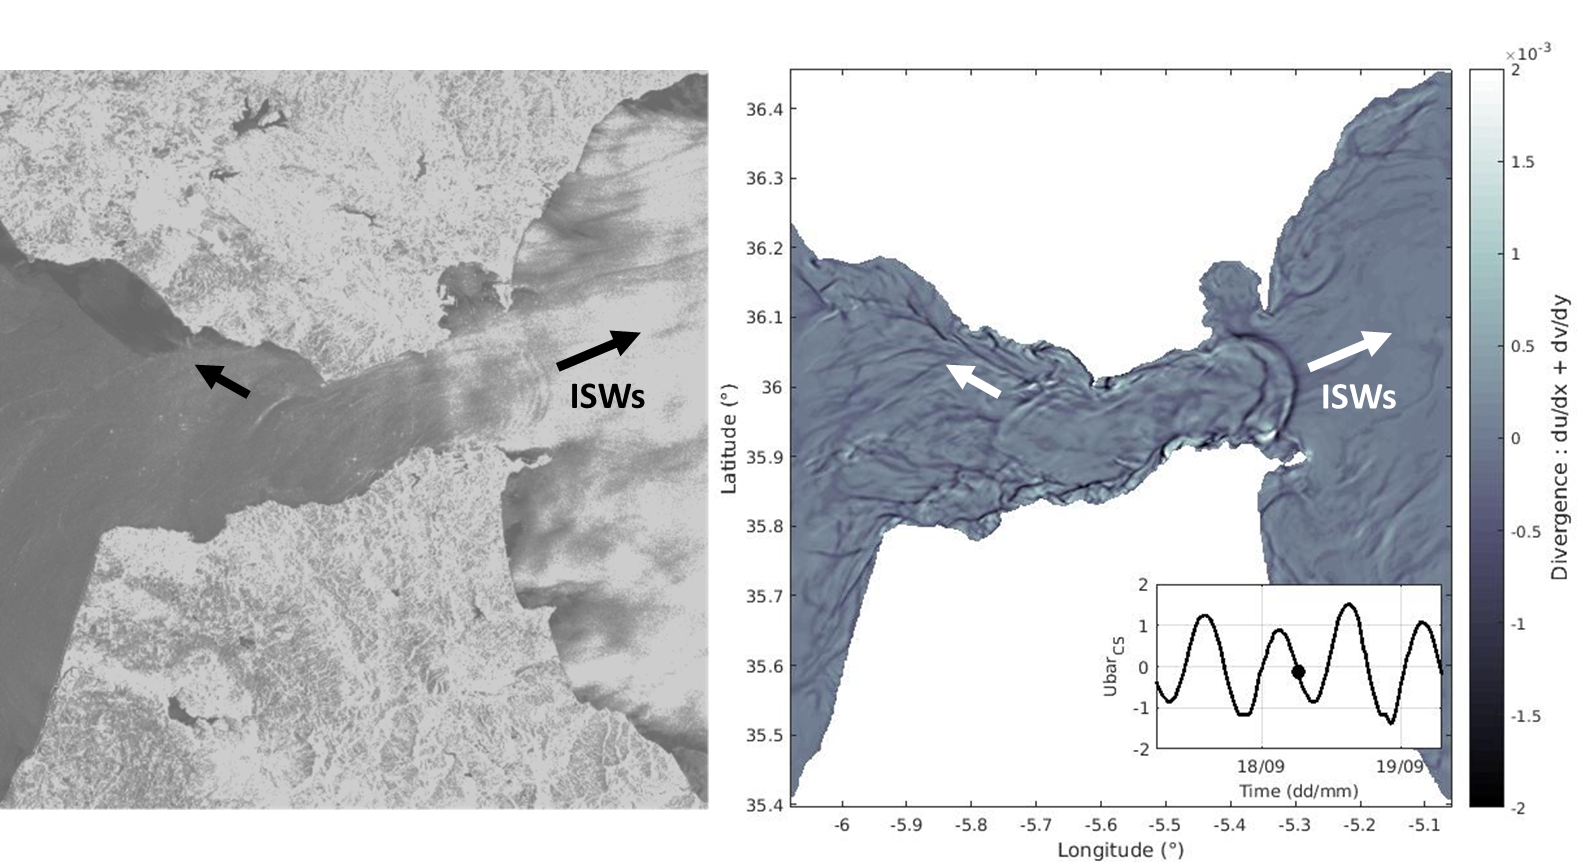
\includegraphics[width=6.3in,height=3.43in]{./media/image3.png}
	\end{Center}

%%%%%%%%%%%%%%%%%%%% Figure/Image No: 3 Ends here %%%%%%%%%%%%%%%%%%%%

\caption{Left – Sentinel-1 Synthetic Aperture Radar (SAR) image acquired on the 18/09/2017 – 06:27:42 and processed by ESA. Right - Divergence of the surface velocity in R\textsubscript{NBQ} the 18/09/2017 – 06:25:00 after a moderate tidal outflow. }
\label{Fig3_Lucie}
\end{figure}

\vspace{\baselineskip}
The RGB image (Figure \ref{Fig5_Lucie} - Left panel) was taken just after the maximum of a moderate tidal outflow when hydraulic jumps are presumably formed in the lee-side of the main sill. On this particular RGB image, instead of the expected single wavefront, two distinct fronts can be observed in CS area : one downstream of CS extending all across the strait and another one located upstream of CS and of smaller extension. At this stage of the tidal cycle, the train of ISWs generated during the previous tidal outflow is still propagating eastward inside the Alboran sea and is made of a larger number of solitary waves than in the above SAR image.\par

\vspace{\baselineskip}
In R\textsubscript{NBQ} (Figure \ref{Fig5_Lucie} - Right), the train of ISWs propagating in the Alboran sea is composed of three solitary waves (still less than on the RGB image). Its propagation speed seems to be well represented, whereas the front deformation is slightly different. 
In R\textsubscript{NBQ}, the two distinct wave fronts observed above CS on the RGB image are located a little further west. At this time in R\textsubscript{NBQ}, the tidal current above CS turned sub-critical and the hydraulic jumps formed above CS have already been released leading to an eastward propagation of the two wave fronts. In so far as some barotropic components (such as N2) are not taken into account in R\textsubscript{NBQ}, it seems that the tidal current above CS is slightly underestimated in R\textsubscript{NBQ}.

\vspace{\baselineskip}


%%%%%%%%%%%%%%%%%%%% Figure/Image No: 4 starts here %%%%%%%%%%%%%%%%%%%%

\begin{figure}[!h]
	\begin{Center}
		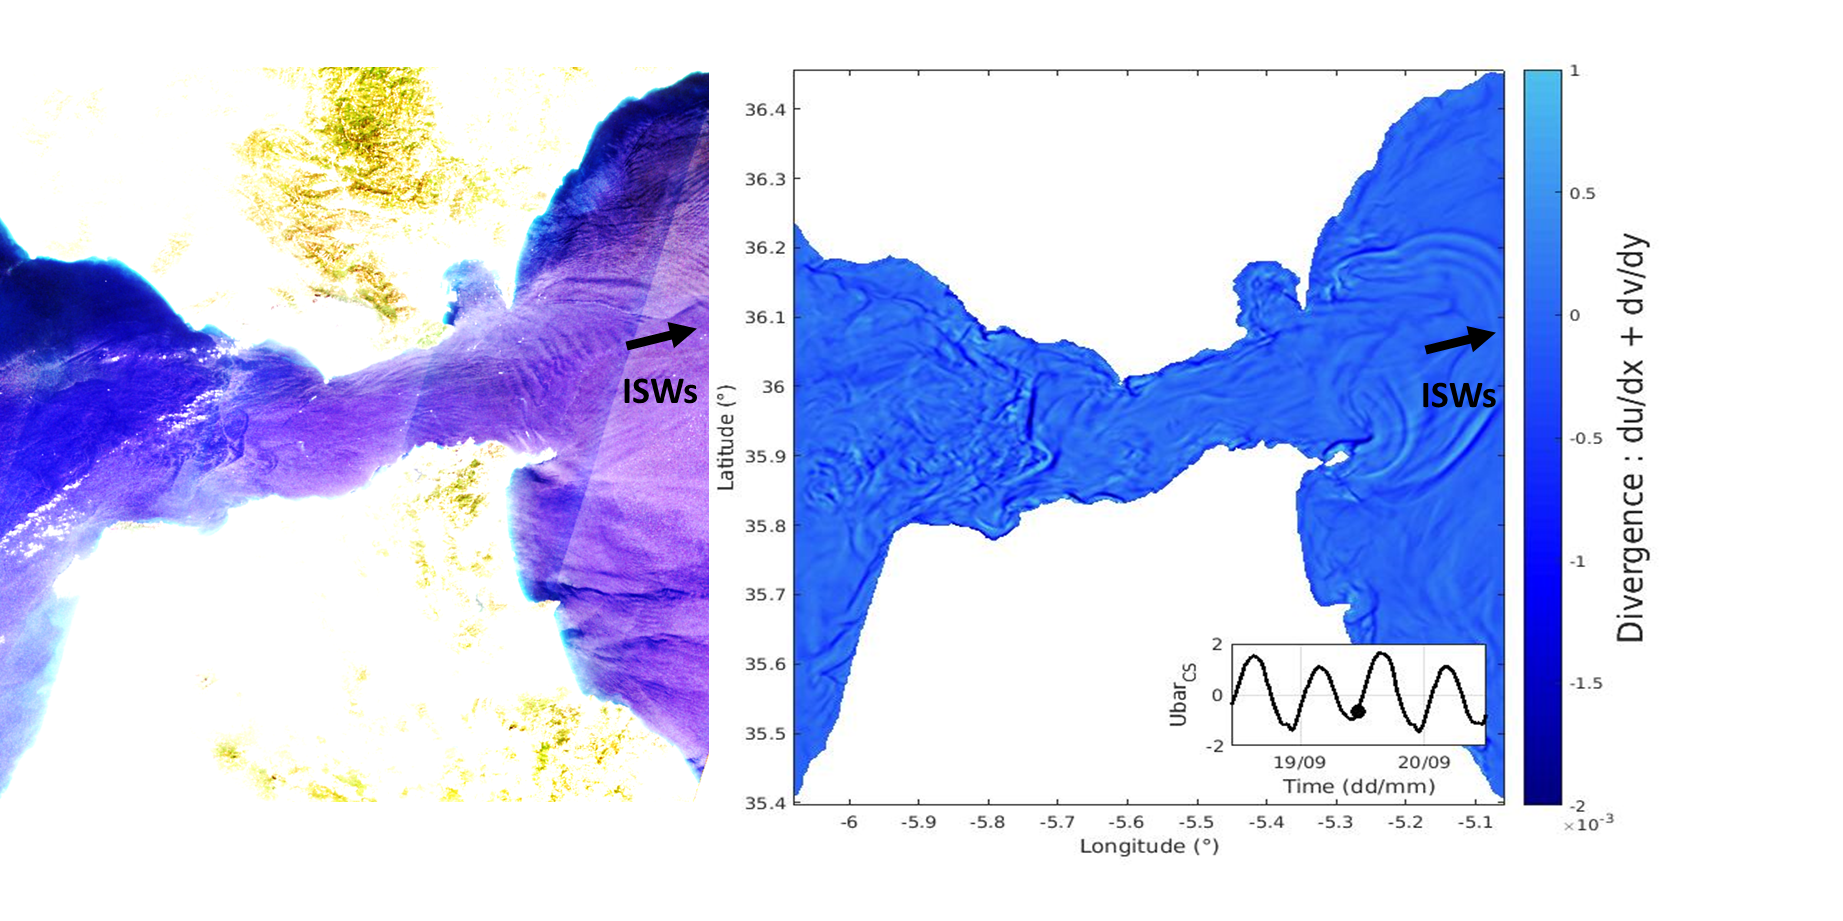
\includegraphics[width=6.3in,height=3.22in]{./media/image4.png}
	\end{Center}

%%%%%%%%%%%%%%%%%%%% Figure/Image No: 4 Ends here %%%%%%%%%%%%%%%%%%%%

\caption{Left - BOA reflectance image (RGB composites) on 19/09/2017 11:18:08, re-processed from Level-2A product for Sentinel-2A/MSI instrument distributed by ESA – Right -  Divergence of the surface velocity in R\textsubscript{NBQ}, the 19/09/2017 – 11:18:00 at a moderate tidal outflow. }
\label{Fig4_Lucie}
\end{figure}

\vspace{\baselineskip}
\subsubsection{Dynamics of the hydraulic jumps}

%%%%%%%%%%%%%%%%%%%% Figure/Image No: 5 starts here %%%%%%%%%%%%%%%%%%%%

\begin{figure}[!h]
	\begin{Center}
		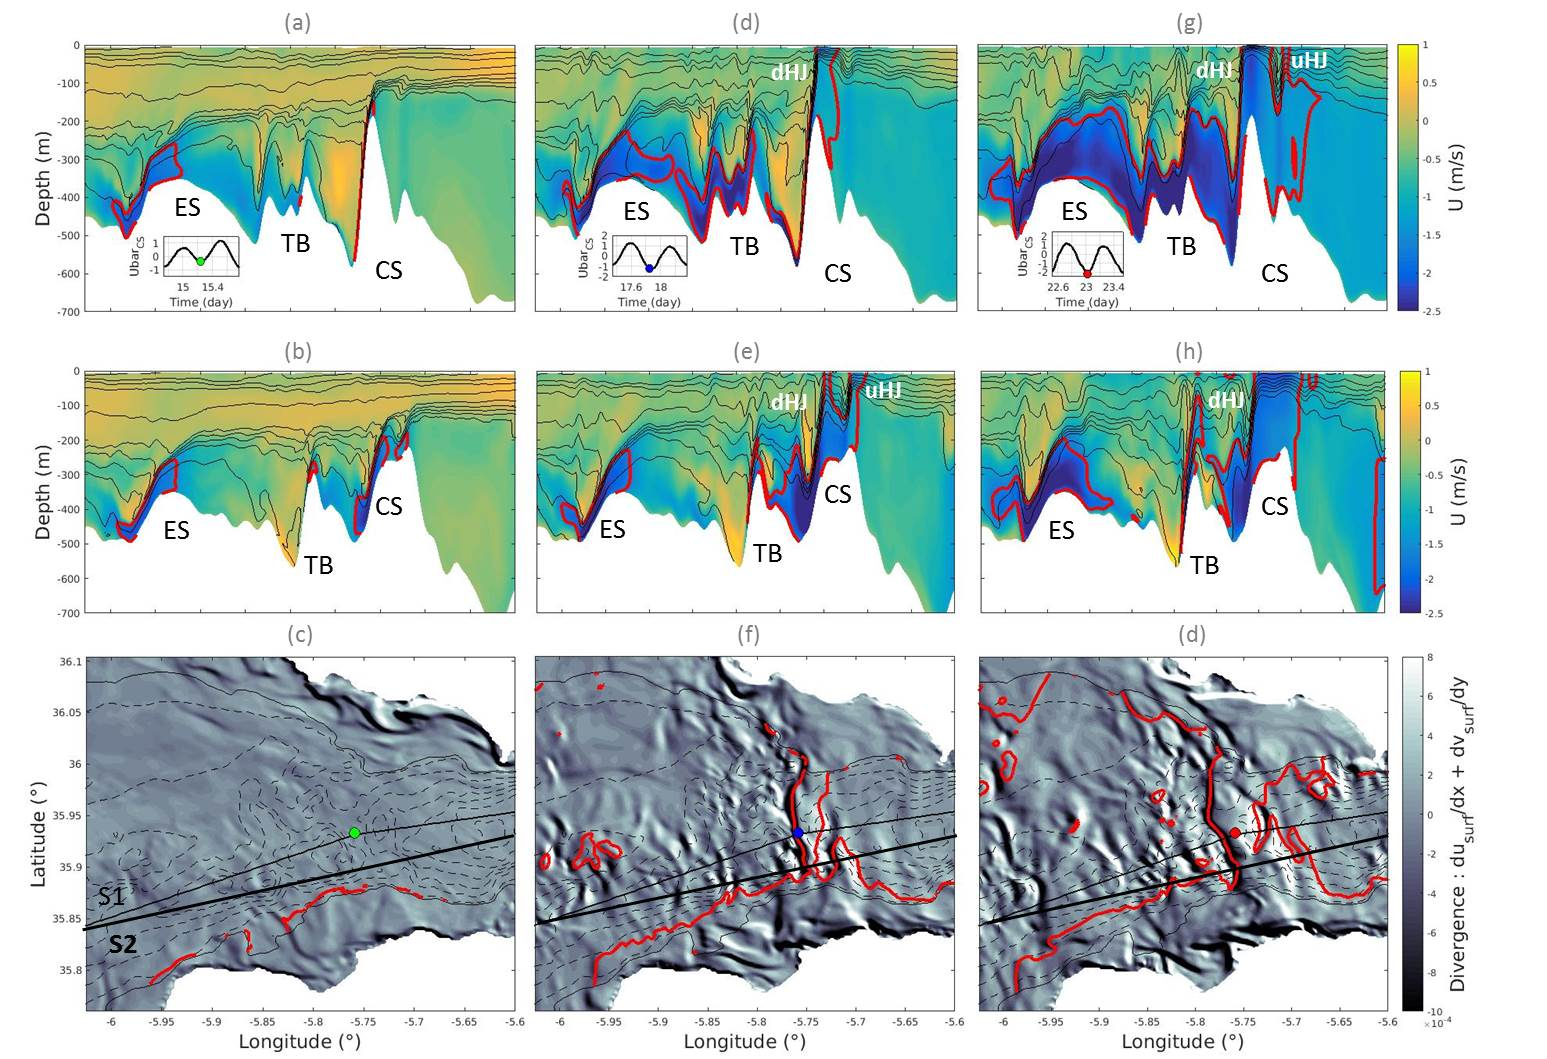
\includegraphics[width=6.61in,height=4.99in]{./media/image5.jpg}
	\end{Center}

%%%%%%%%%%%%%%%%%%%% Figure/Image No: 5 Ends here %%%%%%%%%%%%%%%%%%%%


\caption{ Lower pannels\ -  Divergence of the flow in \textbf{R\textsubscript{NBQ}} at the maximum of a weak tidal outflow (c), a moderate tidal outflow (f) and a strong tidal outflow (d). The black line locates the vertical section 1 (S1) and section 2 (S2). Middle pannels - Section 2 (S2) of the horizontal velocity field in \textbf{R\textsubscript{NBQ}} at the maximum of a weak tidal outflow (b), a moderate tidal outflow (e) and a strong tidal outflow (h). Upper pannels - Section 1 (S1) of the horizontal velocity field in \textbf{R\textsubscript{NBQ}} at the maximum of a weak tidal outflow (a), a moderate tidal outflow (d) and a strong tidal outflow (g). Red contour represent super-critical flow area (F1=c1).}
\label{Fig5_Lucie}
\end{figure}

\vspace{\baselineskip}
Under weak tidal forcing, only a small part of the bottom layer is super-critical above CS crest (partial hydraulic control figure \ref{Fig5_Lucie}.a-b). The surface layer remains sub-critical and there is no signature of any hydraulic jumps at the ocean surface (figure \ref{Fig5_Lucie}.c). \par

\vspace{\baselineskip}
Under moderate tidal forcing (figure \ref{Fig5_Lucie}.d-e), the whole water column is super-critical above CS (total hydraulic control) leading to the formation of large hydraulic jumps. The signature of these hydraulic jumps is visible on the divergence of the surface flow (figure \ref{Fig5_Lucie}.f). We can indeed observe a strong asymmetry between the northern and southern parts of the strait (due to geographical constriction) :\par

\begin{itemize}
	\item in the northern part (figure \ref{Fig5_Lucie}.d), we observe a single super-critical area above CS,\par

	\item in the southern part (figure \ref{Fig5_Lucie}.c), we observe two distinct super-critical regions above CS.
\end{itemize}\par

Hence a moderate tidal outflow is characterized by the formation of two hydraulic jumps: one located downstream of CS extending all across the strait and one located upstream of CS and confined to the southern half section of the strait\par

\vspace{\baselineskip}
Under strong tidal forcing (spring tides), when the outflow is maximal, the southern upstream hydraulic jump (located initially around\  -5.73$ ^{\circ} $ \ of longitude) is swept down to the lee side of the sill (around  -5.76$ ^{\circ} $  of longitude), and in the southern part of the strait, the flow acquires the hydraulic configuration of a pure approach-controlled state, with only one supercritical region extending from the upstream control section to a few hundred meters downstream (of CS).\par

\vspace{\baselineskip}
\subsubsection{ ISWs formation: a strong neap-spring tide variability}

\vspace{\baselineskip}
 During moderate tides (figure \ref{Fig7_Lucie}.b-e), in the middle part of the strait (section 1), an internal hydraulic jump is formed on the downstream side of CS at maximum tidal ouflow. When the tidal flow reverses, the hydraulic jump is released and leads to the eastward propagation of an internal bore (IB). It is then subject to multiple reflections (rW) in Tarrifa Narrows and degenerates into solitary waves (ISWs).\par

\vspace{\baselineskip}
However, during weak neap-tides (figure \ref{Fig7_Lucie}.a-d); the favorable hydraulic conditions for the generation of lee waves (LWs) in the lee-side of CS inhibit the internal bore generation.  \par


\vspace{\baselineskip}
During spring tides (figure \ref{Fig7_Lucie}.c-f), in the middle part of the strait, two internal hydraulic jumps are formed above CS: one upstream (uHJ) and another downstream (dHJ) of the sill. When the tidal flow reverses, the hydraulic jumps are released and lead to the eastward propagation of two internal bores (IB). The largest internal bore (emitted on the downstream side) propagates faster and catches up the smallest one (emitted on the upstream side). It is then subject to multiple reflections (rW) in Tarrifa Narrows and degenerates into solitary waves (ISWs).\par

\vspace{\baselineskip}

\vspace{\baselineskip}

\vspace{\baselineskip}


%%%%%%%%%%%%%%%%%%%% Figure/Image No: 6 starts here %%%%%%%%%%%%%%%%%%%%

\begin{figure}[!h]
	\begin{Center}
		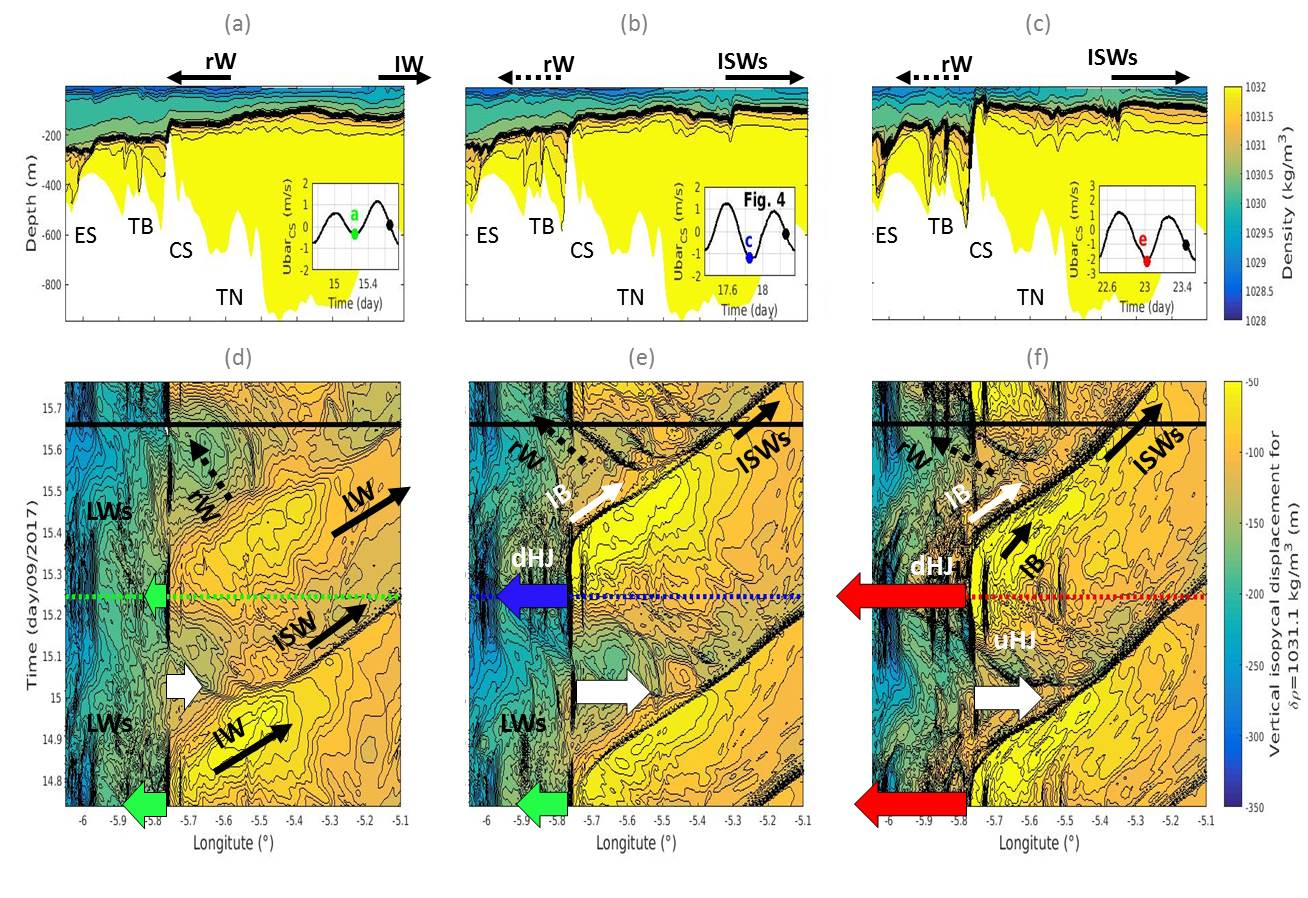
\includegraphics[width=6.3in,height=4.32in]{./media/image6.jpg}
	\end{Center}

%%%%%%%%%%%%%%%%%%%% Figure/Image No: 6 Ends here %%%%%%%%%%%%%%%%%%%%

\caption{ Upper panels \textbf{- }Section 1 of the density field in \textbf{R\textsubscript{NBQ}} after a weak tidal outflow (a), a moderate tidal outflow (b) and a strong tidal outflow (c). Lower panels - Space-time diagram of the vertical isopycnal displacement for $ \rho $ =1031.1 kg/m3 (bold black line on the upper panels) along the section 1 during two weak tidal cycle (a), a moderate and a weak tidal cycle (b) and two strong tidal cycle (c). The white arrows represent the mean tidal inflow above Camarinal sill whereas colored arrows represent the mean tidal outflow above Camarinal sill (green for weak, blue for moderate and red for strong). Horizontal black lines locate temporally the vertical section of the density field (upper panels) whereas colored dotted\ lines locate temporally the maximum of the previous tidal outflow (section 1 on Fig.  \ref{Fig5_Lucie}). }
\label{Fig7_Lucie}
\end{figure}

%\vspace{\baselineskip}

%\printbibliography
%\end{document}

